\qrchapter{https://forgottenpillar.com/rsc/en-fp-chapter1}{The historical context}


\qrchapter{https://forgottenpillar.com/rsc/es-fp-chapter1}{El contexto histórico}


Ellen White recalled encountering the same sentiments in \textit{The Living Temple} that she had warned against early in her ministry:


Elena White recordó haber encontrado los mismos sentimientos en \textit{The Living Temple} contra los que había advertido al principio de su ministerio:


\egw{As we read \normaltext{[The Living Temple]}, I recognized the very sentiments against which I had been bidden to speak in warning \textbf{during the early days of my public labors}. \textbf{When I first left \underline{the State of Maine, it was to go through Vermont and Massachusetts}}, to bear a testimony \textbf{against these sentiments}. ‘Living Temple’ contains the alpha of these theories. I knew that the omega would follow in a little while; and I trembled for our people. I knew that I must warn our brethren and sisters \textbf{not to enter into controversy over \underline{the presence and personality of God}}. The statements made in ‘Living Temple’ in regard to this point are incorrect. The scripture used to substantiate the doctrine there set forth, is scripture misapplied.}[SpTB02 53.2; 1904][https://egwwritings.org/read?panels=p417.271]


\egw{Al leer \normaltext{[The Living Temple]}, reconocí los mismos sentimientos contra los cuales se me había ordenado hablar en advertencia \textbf{durante los primeros días de mis labores públicas}. \textbf{Cuando salí por primera vez \underline{del Estado de Maine, fue para ir por Vermont y Massachusetts}}, para dar un testimonio \textbf{contra estos sentimientos}. ‘Living Temple’ contiene el alfa de estas teorías. Sabía que el omega seguiría en poco tiempo; y temblaba por nuestro pueblo. Sabía que debía advertir a nuestros hermanos y hermanas \textbf{que no entraran en controversia sobre \underline{la presencia y personalidad de Dios}}. Las declaraciones hechas en ‘Living Temple’ con respecto a este punto son incorrectas. Las escrituras utilizadas para fundamentar la doctrina allí expuesta, son escrituras mal aplicadas.}[SpTB02 53.2; 1904][https://egwwritings.org/read?panels=p417.271]


She pinpointed her first encounter with these views: \egwinline{When I first left \textbf{the State of Maine}, it was to go through Vermont and Massachusetts, \textbf{to bear a testimony against these sentiments.}} Her biography, written by her grandson Arthur Lacey White, provides further context on these sentiments. In \textit{Ellen White: The Early Years}, under the section \textit{Wrestling with the Views of the Spiritualizers}, her experiences in eastern Maine reveal more about the controversy over the personality of God and its implications.


Ella señaló su primer encuentro con estas opiniones: \egwinline{Cuando salí por primera vez \textbf{del Estado de Maine}, fue para ir por Vermont y Massachusetts, \textbf{para dar un testimonio contra estos sentimientos.}} Su biografía, escrita por su nieto Arthur Lacey White, proporciona más contexto sobre estos sentimientos. En \textit{Ellen White: The Early Years}, bajo la sección \textit{Luchando con las opiniones de los espiritualizadores}, sus experiencias en el este de Maine revelan más sobre la controversia sobre la personalidad de Dios y sus implicaciones.


\othersQuote{\textbf{\underline{In eastern Maine} Ellen was traveling} and working \textbf{in the atmosphere of the spiritualizers who had \underline{allegorized away heaven, God, Jesus, and the Advent hope}}. In the vision at Exeter in mid-February she seemed to be \textbf{in the presence of Jesus, and she was eager to procure answers to some \underline{vital questions}}.}[ALW, 1BIO 79.4; 1985][https://egwwritings.org/read?panels=p668.582]


\othersQuote{\textbf{\underline{En el este de Maine} Elena estaba viajando} y trabajando \textbf{en la atmósfera de los espiritualizadores que habían \underline{alegorizado el cielo, Dios, Jesús y la esperanza adventista}}. En la visión de Exeter a mediados de febrero, ella parecía estar \textbf{en la presencia de Jesús, y estaba ansiosa por obtener respuestas a algunas \underline{preguntas vitales}}.}[ALW, 1BIO 79.4; 1985][https://egwwritings.org/read?panels=p668.582]


\othersQuoteNoGap{I asked Jesus if \textbf{His Father had a form like Himself}. \textbf{He said He had}, but I could not behold it, for said He, ‘If you should once behold the glory of \textbf{His person}, you would cease to exist.’—Early Writings, 54.}[ALW, 1BIO 79.5; 1985][https://egwwritings.org/read?panels=p668.583]


\othersQuoteNoGap{Le pregunté a Jesús si \textbf{Su Padre tenía una forma como Él}. \textbf{Él dijo que sí la tenía}, pero que yo no podía contemplarla, porque, dijo Él: ‘Si alguna vez contemplases la gloria de \textbf{Su persona}, dejarías de existir.’—Primeros Escritos, 54.}[ALW, 1BIO 79.5; 1985][https://egwwritings.org/read?panels=p668.583]


\othersQuoteNoGap{This was not the only occasion Ellen was to converse with Jesus and the angel \textbf{about the \underline{person of Jesus} and concerning \underline{God being a personal being}}. \textbf{\underline{The answers satisfied her fully that the spiritualizers were in gross error}}.}[ALW, 1BIO 80.1; 1985][https://egwwritings.org/read?panels=p668.586]


\othersQuoteNoGap{Esta no fue la única ocasión en que Elena conversó con Jesús y el ángel \textbf{acerca de la \underline{persona de Jesús} y concerniente a \underline{Dios siendo un ser personal}}. \textbf{\underline{Las respuestas la satisficieron plenamente de que los espiritualizadores estaban en grave error}}.}[ALW, 1BIO 80.1; 1985][https://egwwritings.org/read?panels=p668.586]


The vision Arthur Lacey White referred to is known as the \textit{vision on the personality of God}, which we will examine later. This vision confirms that the doctrine of the \emcap{personality of God} teaches that God the Father has a form, just as Jesus does. It specifically addresses the \others{\textbf{person of Jesus} and concerning \textbf{God being a personal being}.}


La visión a la que Arthur Lacey White se refirió es conocida como la \textit{visión sobre la personalidad de Dios}, que examinaremos más adelante. Esta visión confirma que la doctrina de la \emcap{personalidad de Dios} enseña que Dios el Padre tiene una forma, así como Jesús la tiene. Aborda específicamente la \others{\textbf{persona de Jesús} y concerniente a \textbf{Dios siendo un ser personal}.}


\begin{figure}[t]
    \centering
    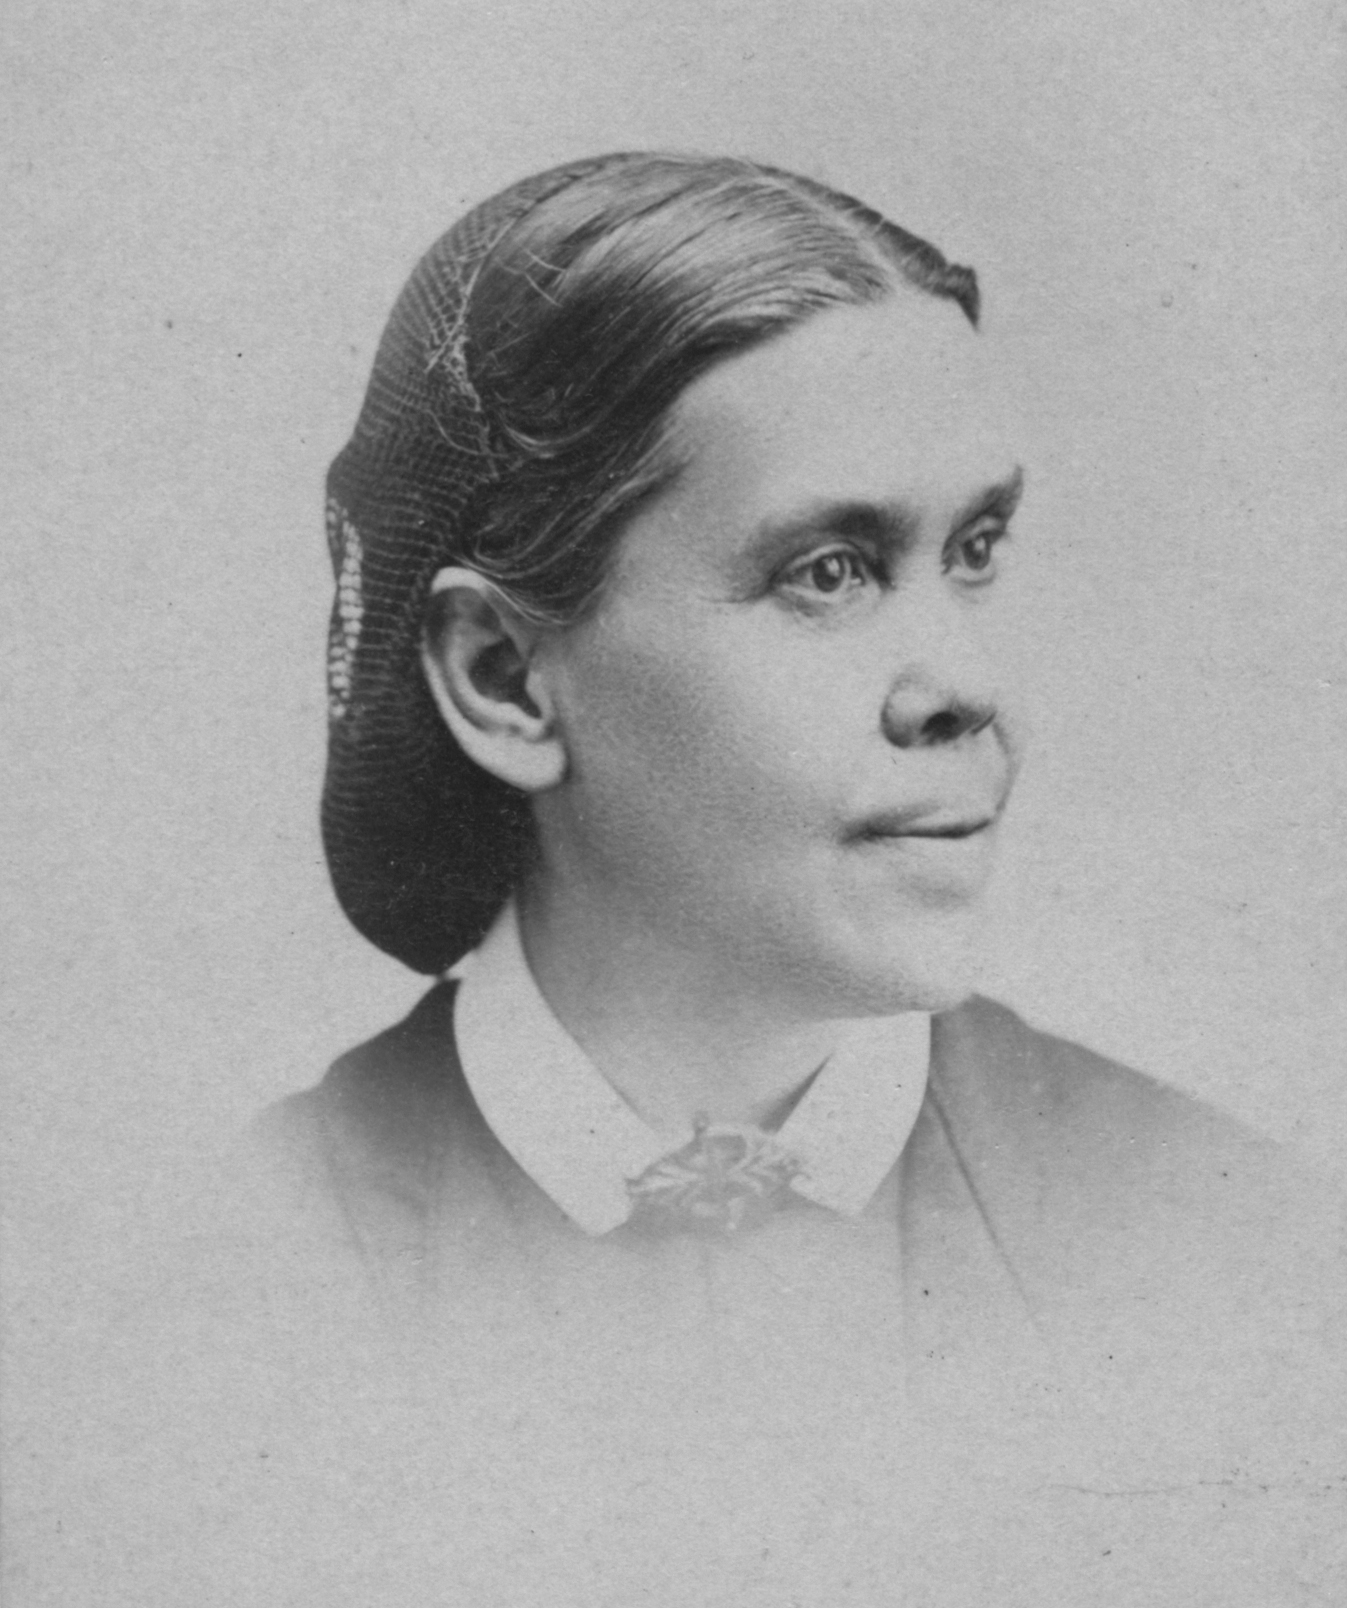
\includegraphics[width=0.65\linewidth]{images/ellen-white.jpg}
    \caption*{Ellen G. White}
    \label{fig:ellen-g-white}
\end{figure}


\begin{figure}[t]
    \centering
    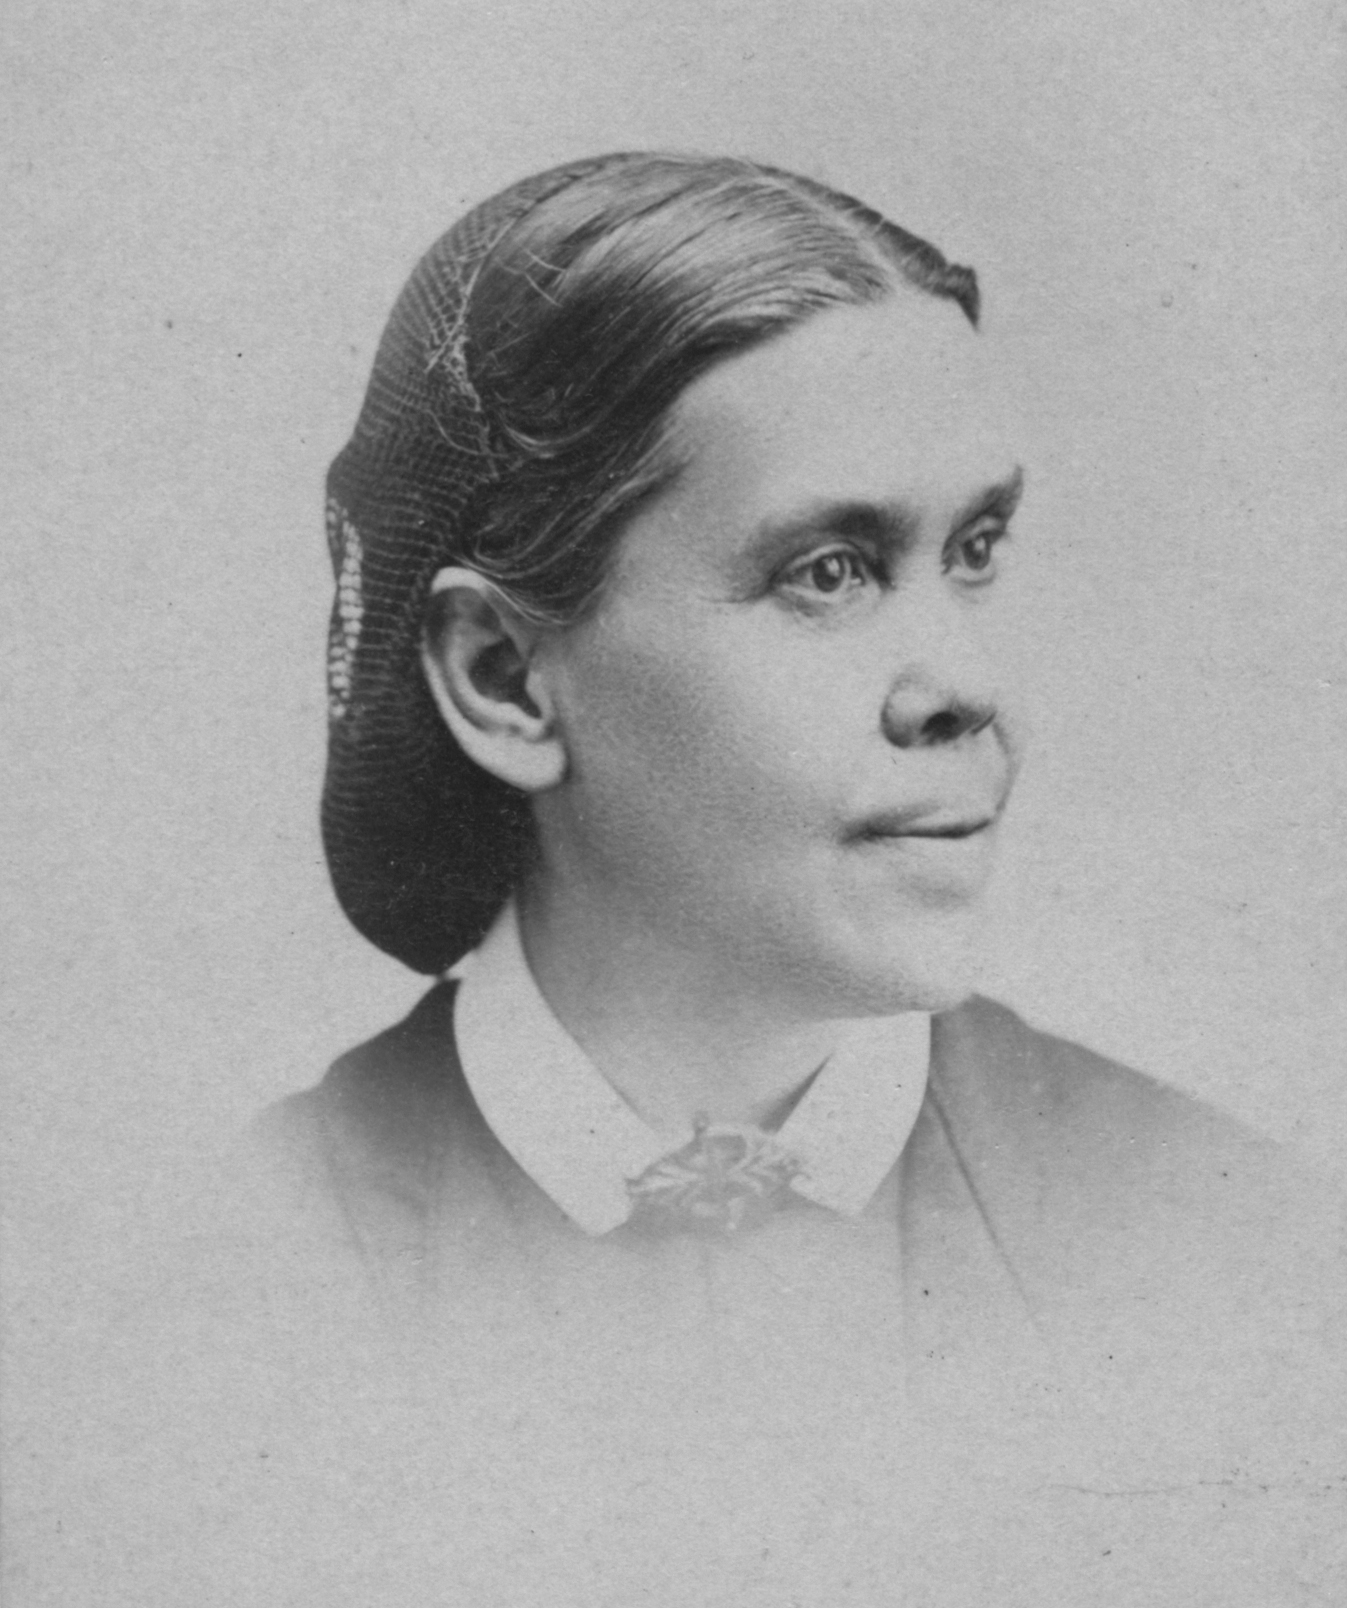
\includegraphics[width=0.65\linewidth]{images/ellen-white.jpg}
    \caption*{Elena G. de White}
    \label{fig:ellen-g-white}
\end{figure}


Consider the first point of the \emcap{Fundamental Principles}, which states that Seventh-day Adventists believe in \others{one God, \textbf{a personal, spiritual being}.}[First point of the Fundamental Principles][https://forgotten-pillar.s3.us-east-2.amazonaws.com/A+declaration+of+the+fundamental+principles+taught+and+practiced+by+the+Seventh-day+Adventists++.pdf] This makes it clear that the central issue in the doctrine of the \emcap{personality of God} concerns the outward, bodily form of the Father. But why was this such a vital and significant question? What were the implications of God having a bodily, personal form?


Considere el primer punto de los \emcap{Principios Fundamentales}, que establece que los Adventistas del Séptimo Día creen en \others{un Dios, \textbf{un ser personal, espiritual}.}[Primer punto de los Principios Fundamentales][https://forgotten-pillar.s3.us-east-2.amazonaws.com/A+declaration+of+the+fundamental+principles+taught+and+practiced+by+the+Seventh-day+Adventists++.pdf] Esto deja claro que el tema central en la doctrina de la \emcap{personalidad de Dios} concierne a la forma exterior, corporal del Padre. Pero, ¿por qué fue esta una pregunta tan vital y significativa? ¿Cuáles fueron las implicaciones de que Dios tuviera una forma corporal y personal?


\othersQuote{But because the pioneers of the Seventh-day Adventist Church held that prophecy was fulfilled on October 22, 1844, and that an important work began in heaven in the Most Holy Place of the heavenly sanctuary at that time, and because the Adventists who had become \textbf{spiritualizers} took the position that Christ had come into their hearts on October 22, 1844, and that His kingdom was in their hearts, the founders of the church, and notably Ellen White, were classed by the world generally, and also by those that SDAs have termed first-day Adventists, as one and the same group. Here again the great enemy cast aspersion upon the true, paralleling it with a false, spurious experience.}[ALW, 1BIO 80.2; 1985][https://egwwritings.org/read?panels=p668.587]


\othersQuote{Pero debido a que los pioneros de la Iglesia Adventista del Séptimo Día sostuvieron que la profecía se cumplió el 22 de octubre de 1844, y que una obra importante comenzó en el cielo en el Lugar Santísimo del santuario celestial en ese momento, y debido a que los adventistas que se habían convertido en \textbf{espiritualizadores} tomaron la posición de que Cristo había entrado en sus corazones el 22 de octubre de 1844, y que Su reino estaba en sus corazones, los fundadores de la iglesia, y notablemente Elena G. de White, fueron clasificados por el mundo en general, y también por aquellos que los ASD han denominado adventistas del primer día, como un mismo grupo. Aquí nuevamente el gran enemigo arrojó calumnias sobre lo verdadero, poniéndolo en paralelo con una experiencia falsa y espuria.}[ALW, 1BIO 80.2; 1985][https://egwwritings.org/read?panels=p668.587]


\othersQuoteNoGap{Ellen White was to speak of this matter again, particularly in the closing paragraphs of her first little book, Experience and Views, published in 1851. As one reads this he will note the use of \textbf{the term spiritualism}, which must be taken in the light of the work of the spiritualizers and not in the light of what today is understood to be spiritualism or spiritism, although both emanate from the same source.}[ALW, 1BIO 80.3; 1985][https://egwwritings.org/read?panels=p668.588]


\othersQuoteNoGap{Elena G. de White hablaría de este asunto nuevamente, particularmente en los párrafos finales de su primer librito, Experience and Views, publicado en 1851. Al leer esto, se notará el uso del \textbf{término espiritualismo}, que debe tomarse a la luz de la obra de los espiritualizadores y no a la luz de lo que hoy se entiende por espiritualismo o espiritismo, aunque ambos emanan de la misma fuente.}[ALW, 1BIO 80.3; 1985][https://egwwritings.org/read?panels=p668.588]


\othersQuoteNoGap{We turn now to the statement written and published in 1851 as found in Ibid., 77, 78:}[ALW, 1BIO 80.4; 1985][https://egwwritings.org/read?panels=p668.589]


\othersQuoteNoGap{Nos dirigimos ahora a la declaración escrita y publicada en 1851 como se encuentra en Ibid., 77, 78:}[ALW, 1BIO 80.4; 1985][https://egwwritings.org/read?panels=p668.589]


\othersQuoteNoGap{\textbf{I have frequently been falsely charged with teaching views peculiar to Spiritualism}. But before the editor of The Day-Star ran into that delusion, \textbf{the Lord \underline{gave me a view} of the sad and desolating effects that would be produced upon the flock by him and others \underline{in teaching the spiritual views}}.}[ALW, 1BIO 80.5; 1985][https://egwwritings.org/read?panels=p668.590]


\othersQuoteNoGap{\textbf{Con frecuencia he sido acusada falsamente de enseñar puntos de vista peculiares al Espiritualismo}. Pero antes de que el editor de The Day-Star cayera en esa ilusión, \textbf{el Señor \underline{me dio una visión} de los tristes y desoladores efectos que serían producidos sobre el rebaño por él y otros \underline{al enseñar las vistas espirituales}}.}[ALW, 1BIO 80.5; 1985][https://egwwritings.org/read?panels=p668.590]


\othersQuoteNoGap{I have often seen the lovely \textbf{Jesus, that He is a person}. I asked Him \textbf{\underline{if His Father was a person} and \underline{had a form} like Himself}. Said Jesus, ‘I am in \textbf{the express image of My Father’s person}.}[ALW, 1BIO 80.6; 1985][https://egwwritings.org/read?panels=p668.591]


\othersQuoteNoGap{A menudo he visto al amado \textbf{Jesús, que Él es una persona}. Le pregunté \textbf{\underline{si Su Padre era una persona} y \underline{tenía una forma} como Él}. Dijo Jesús: ‘Yo soy \textbf{la imagen misma de su sustancia}.}[ALW, 1BIO 80.6; 1985][https://egwwritings.org/read?panels=p668.591]


\othersQuoteNoGap{\textbf{I have often seen that \underline{the spiritual view} took away all the glory of heaven, and that in many minds the throne of David and the lovely person of Jesus have been burned up in the fire of Spiritualism.} I have seen that some who have been deceived and led into this error will be brought out into the light of truth, but it will be almost impossible for them to get entirely rid of \textbf{the deceptive power of Spiritualism}. Such should make thorough work in confessing their errors and leaving them forever.}[ALW, 1BIO 80.7; 1985][https://egwwritings.org/read?panels=p668.592]


\othersQuoteNoGap{\textbf{A menudo he visto que \underline{la vista espiritual} quitaba toda la gloria del cielo, y que en muchas mentes el trono de David y la hermosa persona de Jesús han sido quemados en el fuego del Espiritualismo.} He visto que algunos que han sido engañados y llevados a este error serán sacados a la luz de la verdad, pero será casi imposible para ellos deshacerse completamente de \textbf{el poder engañoso del Espiritualismo}. Tales personas deberían hacer una obra completa en confesar sus errores y abandonarlos para siempre.}[ALW, 1BIO 80.7; 1985][https://egwwritings.org/read?panels=p668.592]


\othersQuoteNoGap{\textbf{The spiritualization of heaven, God, Christ, and the coming of Christ lay at the foundation of much of the fanatical teachings that 17-year-old Ellen Harmon was called upon by God to meet in those formative days. The visions firmly established \underline{the personality of God and Christ}, \underline{the reality of heaven} and the reward to the faithful, and the resurrection. This sound guidance saved the emerging church}.}[ALW, 1BIO 81.1; 1985][https://egwwritings.org/read?panels=p668.595]


\othersQuoteNoGap{\textbf{La espiritualización del cielo, Dios, Cristo y la venida de Cristo estaba en la base de gran parte de las enseñanzas fanáticas que Dios llamó a Elena Harmon, de 17 años, a enfrentar en aquellos días formativos. Las visiones establecieron firmemente \underline{la personalidad de Dios y Cristo}, \underline{la realidad del cielo} y la recompensa a los fieles, y la resurrección. Esta sólida guía salvó a la iglesia emergente}.}[ALW, 1BIO 81.1; 1985][https://egwwritings.org/read?panels=p668.595]


The mistake of the Millerite movement in 1844 lay in misunderstanding the nature of the event, not its timing. Daniel 7:13-14 describes Christ coming to the Ancient of Days in heaven to receive dominion, glory, and a kingdom—not His second coming to earth. This event, marking the beginning of Christ’s work in the Most Holy Place, occurred at the conclusion of the 2300-day prophecy in 1844. Unlike other Adventist groups, the emerging Seventh-day Adventist Church uniquely recognized this heavenly event.


El error del movimiento millerita en 1844 radicaba en la incomprensión de la naturaleza del evento, no de su tiempo. Daniel 7:13-14 describe a Cristo viniendo al Anciano de Días en el cielo para recibir dominio, gloria y un reino—no Su segunda venida a la tierra. Este evento, que marca el comienzo de la obra de Cristo en el Lugar Santísimo, ocurrió al concluir la profecía de los 2300 días en 1844. A diferencia de otros grupos adventistas, la emergente Iglesia Adventista del Séptimo Día reconoció de manera única este evento celestial.


This understanding is built on key premises:
\begin{itemize}
    \item Heaven is a real, literal place (John 14:1-3).
    \item There is a literal sanctuary in heaven where Christ ministers (Hebrews 8:2). 
    \item A real, physical throne exists in this sanctuary, occupied by God Himself (Daniel 7:9-10; Revelation 4:2-3; Ezekiel 1:26-28; Psalm 11:4).
\end{itemize}


Esta comprensión se basa en premisas clave:
\begin{itemize}
    \item El cielo es un lugar real y literal (Juan 14:1-3).
    \item Existe un santuario literal en el cielo donde Cristo ministra (Hebreos 8:2). 
    \item Un trono real y físico existe en este santuario, ocupado por Dios mismo (Daniel 7:9-10; Apocalipsis 4:2-3; Ezequiel 1:26-28; Salmo 11:4).
\end{itemize}


Why is the question of the Father’s bodily form so important? If God were not a physical being, there would be no need for a literal throne, sanctuary, or heavenly ministry. A spiritualized interpretation undermines the foundation of Seventh-day Adventist theology, leading to a domino effect that erodes the doctrine of Christ’s priestly work.


¿Por qué es tan importante la cuestión de la forma corporal del Padre? Si Dios no fuera un ser físico, no habría necesidad de un trono literal, un santuario o un ministerio celestial. Una interpretación espiritualizada socava el fundamento de la teología Adventista del Séptimo Día, llevando a un efecto dominó que erosiona la doctrina de la obra sacerdotal de Cristo.


The doctrine of the \emcap{personality of God} was a simple yet foundational teaching, affirmed in the first point of the \emcap{Fundamental Principles}: \textit{“One God, a personal, spiritual being.”} As such, He is not omnipresent by Himself but through His representative, the Holy Spirit.\footnote{The first point of the Fundamental Principles: \othersQuote{That there is \textbf{one God}, \textbf{a \underline{personal, spiritual being}}, the creator of all things, omnipotent, … and \textbf{everywhere present by \underline{his representative}, the Holy Spirit}. Ps. 139:7.}} When Ellen White asked Jesus \egwinline{if His Father \textbf{was a person} and \textbf{had a \underline{form}} like Himself,}[EW 77.1; 1882][https://egwwritings.org/read?panels=p28.490&index=0] we see clearly that the \textit{outward bodily \textbf{form}} is \textit{the quality or state} defining God as a person. This understanding was central in addressing the Kellogg crisis regarding \textit{The Living Temple}, which deviated from this core belief.


La doctrina de la \emcap{personalidad de Dios} era una enseñanza simple pero fundamental, afirmada en el primer punto de los \emcap{Principios Fundamentales}: \textit{“Un Dios, un ser personal y espiritual.”} Como tal, Él no es omnipresente por Sí mismo sino a través de Su representante, el Espíritu Santo.\footnote{El primer punto de los Principios Fundamentales: \othersQuote{Que hay \textbf{un Dios}, \textbf{un \underline{ser personal y espiritual}}, el creador de todas las cosas, omnipotente, … y \textbf{presente en todas partes por \underline{su representante}, el Espíritu Santo}. Sal. 139:7.}} Cuando Elena G. de White le preguntó a Jesús \egwinline{si Su Padre \textbf{era una persona} y \textbf{tenía una \underline{forma}} como Él mismo,}[EW 77.1; 1882][https://egwwritings.org/read?panels=p28.490&index=0] vemos claramente que la \textit{externa \textbf{forma} corporal} es \textit{la cualidad o estado} que define a Dios como persona. Esta comprensión fue central para abordar la crisis de Kellogg con respecto a \textit{The Living Temple}, que se desviaba de esta creencia fundamental.


But do our current \textit{Fundamental Beliefs} still affirm this doctrine? Do they explicitly teach that God is a real person with a bodily form, whose literal presence is in heaven, while He is omnipresent through His Spirit? The doctrine of God’s presence and personality is absent from today’s official beliefs. While individually, we may still believe in it, why was such a vital teaching omitted? What were the reasons behind this shift? These are the questions we must explore further in the context of \textit{The Foundation of Our Faith}.


Pero, ¿nuestras actuales \textit{creencias fundamentales} todavía afirman esta doctrina? ¿Enseñan explícitamente que Dios es una persona real con forma corporal, cuya presencia literal está en el cielo, mientras que Él es omnipresente a través de Su Espíritu? La doctrina de la presencia y personalidad de Dios está ausente de las creencias oficiales actuales. Aunque individualmente, todavía podemos creer en ella, ¿por qué se omitió una enseñanza tan vital? ¿Cuáles fueron las razones detrás de este cambio? Estas son las preguntas que debemos explorar más a fondo en el contexto de \textit{El Fundamento de Nuestra Fe}.


% The Historical Context

\begin{titledpoem}
    
    \stanza{
        By visions Ellen White stood firm, \\
        Against false views; she did affirm. \\
        The Father’s form, a truth profound, \\
        In this essential faith was found.
    }

    \stanza{
        "Spiritualizers" sought to claim \\
        That heaven’s realm was but a name. \\
        Yet God has form, like Christ His Son, \\
        This truth our founders built upon.
    }

    \stanza{
        A Spirit Person God does reign \\
        The universe is His domain \\
        This doctrine once our cornerstone, \\
        Has somehow from our statements flown.
    }
    
\end{titledpoem}


% % The Historical Context
\begin{titledpoem}
    \stanza{
        Młoda Ellen przez Maine wędrowała, \\
        Przed błędnymi poglądami ostrzegała. \\
        Bóg ma postać, jak Chrystus objawił, \\
        I ten fakt w wizji Pan jej przedstawił.
    }

    \stanza{
        Spirytualista koncepcję swą sieje, \\
        Że fizyczne niebo wcale nie istnieje. \\
        Lecz osobowość Boga to nie abstrakcja pusta, \\
        To prawda, którą głosiły już pionierów usta.
    }

    \stanza{
        Alfa błędu w „Living Temple” się zjawiła, \\
        Omega wkrótce potem nastąpiła. \\
        Czy ta doktryna, niegdyś tak jasna, \\
        W naszych wierzeniach już nie wygasła?
    }
\end{titledpoem}

